\chapter{Composants de base d'un assistant personnel}

\section{Introduction}
\paragraph{}
Dans ce chapitre, nous détaillerons un peu plus l'aspect technique d'une architecture typique d'un SPA (Speech Personal Assistant). Nous commencerons d'abord par définir des notions de base. Nous ne  traiterons que celles qui ont été les plus utilisées dans les travaux que nous avons examiné. La suite du chapitre sera organisée en sections qui décrirons chacune le fonctionnement d'une partie du SPA, en citant les travaux et références qui relatent de cette dernière. Nous terminerons sur une conclusion qui introduira le chapitre suivant.

\section{Schéma global d'un SPA}
\label{spaSchemSection}
\paragraph{}
Durant nos lectures des différents travaux sur le domaine, nous avons pu dresser un schéma assez général qui englobe les principaux modules d'un SPA : 
\begin{figure}[H]
	\centering
	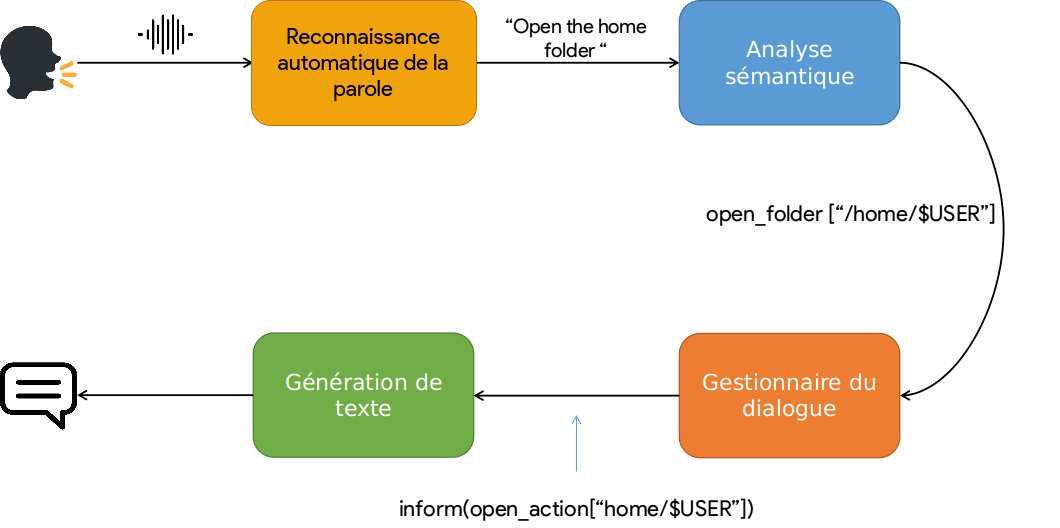
\includegraphics[width=0.8\linewidth]{images/SPA_diagram_2.png}
	\caption{Schéma abstractif d'un SPA \citep{spa_arch}}
	\label{fig:spaDiagram}
\end{figure}
\paragraph{}
Le processus peut être résumé en des étapes cruciales (qui seront détaillées dans les sections suivantes) : 
\begin{itemize}
	\label{spaLifeCycle}
	\item L'utilisateur énonce une requête en utilisant sa voix. Le signal est ensuite transformé en sa version textuelle.
	\item Étant sous un format textuel brut, la requête ne peut pas être interprétée ou comprise par la machine. Une représentation sémantique est générée qui regroupera les principales informations contenues dans la requête, à savoir l'intention de l'utilisateur et ses arguments.
	\item Au fur et à mesure que l'utilisateur énonce des requêtes, le système doit pouvoir être capable d'utiliser le contexte du dialogue pour interagir avec ce dernier afin d'atteindre le but final du dialogue (exécuter une commande système, trouver des informations internet ou sur la machine locale, etc.). Le gestionnaire du dialogue communique avec son environnement en utilisant la même représentation sémantique produite par l'analyse précédente.
	\item Puisqu'il est préférable de cacher à l'utilisateur tout comportement interne au système, il serait préférable de transformer la trame sémantique (voir la figure ~\ref{fig:semanticFrame}) en texte naturel pour l'afficher en sortie.
\end{itemize}
\paragraph{}
Il est à noter que chacun des modules seront indépendants pour ce qu'il est de leur fonctionnement interne. Ainsi, aucun n'assumera un fonctionnement arbitraire des autres modules. Seul le format des informations qui circulent entre eux devra être établi au préalable pour un fonctionnement durable et robuste au changement.
\paragraph{}
Pour ce qui est de la suite du chapitre, nous allons présenter les différents modules ainsi que les techniques et architectures qui sont considérées comme étant l'état de l'art du domaine. 

\section{Notions et aspects théoriques}
\paragraph{}
Dans cette section, nous présenterons différentes notions liées au domaine de l'apprentissage automatique, pour ensuite les citer dans les modules qui les utilisent. 
\subsection{Apprentissage automatique}
\paragraph{}
Le plus souvent, un domaine scientifique peut être défini à travers le ou les types de problèmes dont il essaye de trouver une solution. D'après \citep{mitchelllearning}, l'auteur définit ce problème sous forme d'une question :
\begin{quote}
	\say{How can we build computer systems that automatically improve with experience, and what are the fundamental laws that govern all learning processes?}\\\citep{mitchelllearning}
\end{quote}
que nous pouvons traduire par :
\begin{quote}
	\say{Comment pourrions nous développer un système informatique qui pourrait s'améliorer à travers l'expérience, et quelles seraient les lois qui régiraient le processus d'apprentissage?}
\end{quote}
\par 
D'après \citep{mitchelllearning}, l'apprentissage automatique est un paradigme qui stipule qu'un système informatique peut apprendre à effectuer un ensemble de tâches T, sachant qu'il dispose d'un ensemble de données E, tout en améliorant sa performance P.
\par
Il existe plusieurs sous-catégories d'apprentissage automatique. Elles diffèrent principalement par la manière dont le système apprend, du type de données sur lesquelles il apprend. ainsi que du but de son apprentissage (classification, régression, etc.). Nous pouvons citer les catégories suivantes :
\begin{itemize}
	\item  \textbf{Apprentissage supervisé} : Les algorithmes de cette catégorie ont besoin d'une assistance externe. Les données doivent être séparées en deux parties (ensemble d'apprentissage et de test). Un \textit{label} (ou classe) est associé à chaque instance pour permettre à l'algorithme de calculer un certain taux d'erreur qu'il essayera de minimiser au fur et à mesure qu'une nouvelle instance lui est présentée \citep{supervised_learning}. Idéalement, le système pourra apprendre une certaine fonction $\hat{f} : X \rightarrow Y$ qui liera les entrées $X$ aux sorties $Y$ en minimisant l'erreur $E_Y$ 
	
	\item \textbf{Apprentissage non supervisé} : Dans ce cas, les algorithmes ne disposent pas d'un étiquetage des données. Ils essayeront donc d'apprendre des \textit{pattern} ou motifs fréquents pour grouper les données similaires. De tels algorithmes ne se préoccupent pas de la classe, mais de la similarité entre un groupe de données et un autre \citep{unsupervised_learning}.
	
	\item \textbf{Apprentissage par renforcement} : Cette dernière catégorie regroupe des algorithmes qui apprennent par un système de \textit{trial and error} (Essais et erreur). C'est à dire qu'en interagissant avec l'environnement, l'agent apprenant (l'algorithme) apprendra à accomplir une tâche précise en exécutant des actions qui modifierons son état et celui de son environnement (voir la section \ref{reinf_learning})
\end{itemize}
\par
Dans les sections suivantes, nous nous intéresserons à quelques types d'algorithme d'apprentissage automatique. 
\subsection{Réseaux de neurones artificiels}
\paragraph{}
Un réseau de neurones artificiels est une structure d'appariement non-linéaire entre un ensemble de caractéristiques en entrée et sortie; ces réseaux sont inspirés de la façon dont les systèmes nerveux biologiques fonctionnent. Ils permettent de modéliser les relations sous-jacentes des données. Ils sont composés d'un nombre arbitrairement large de petites unités de calcul interconnectées appelées neurones, qui traitent l'information d'une manière parallèle dans le but de résoudre un problème bien spécifique \citep{neural_nets}. Ils ont notamment connu un très grand succès pendant les dernières années dans différents domaines comme la reconnaissance d'images \citep{inception}, la reconnaissance automatique de la parole \citep{speech_reco_dnn,speech_reco_Yu2015} ou encore la classification de textes \citep{seq2seq_multitask_classification,dnn_text_classification}.
\par 
Il existe une variété d'architectures de réseaux de neurones. Nous traiterons dans cette section trois d'entre elles : 
\begin{itemize}
	\item Réseaux de neurones multicouches denses
	\item Réseaux de neurones profonds
	\item Réseaux de neurones récurrents et leurs variantes
\end{itemize}
\subsubsection{Réseaux de neurones multicouches denses}

\paragraph{}
La forme la plus basique que peut avoir un réseau de neurones est celle d'un réseau multicouches comme montré dans la figure \ref{mlp}. Elle se compose de trois parties :
\begin{itemize}
	\item \textbf{Une couche d'entrée :} Elle reçoit l'information en entrée codifié en un vecteur numérique $\chi$
	
	\item  \textbf{Une ou plusieurs couches cachées :} le c\oe{}ur du réseau, c'est une succession de couches de neurones où chaque couche $C_i$ reçoit un signal sous forme d'une ou plusieurs valeurs numériques depuis une couche antérieure $C_{i-1}$ ou bien la couche d'entrée $\chi$, puis envoit en sortie un autre signal de même nature qui est une combinaison non-linéaire du signal en entrée vers une couche cachée suivante $C_{i+1}$ ou bien la couche de sortie
	\item \textbf{Une couche de sortie :}
	elle permet de calculer une valeur $\hat{y}$ qui peut être vue comme la prédiction du modèle $\Phi$ par rapport à son entrée $\chi$ : 
	\begin{equation}
	\hat{y} = f_\Phi(\chi)
	\end{equation}
\end{itemize}
Le réseau calcule une erreur $e(y,\hat{y})$ en fonction de sa valeur en sortie et de la valeur exacte puis corrigera cette erreur au fur et à mesure du parcours des données d'apprentissage \citep{mlp}
\begin{figure}[H]
	\centering
	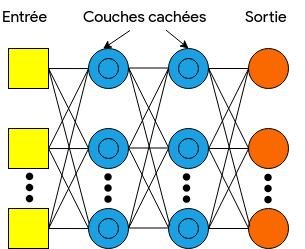
\includegraphics[width=0.5\linewidth]{images/notions/mlp.png}
	\caption{Architecture basique d'un réseau de neurones multicouches}
	\label{mlp}
\end{figure}

\subsubsection{Réseaux de neurones profonds}\label{part2DNN}
\paragraph{}
Les réseaux de neurones à une seule couche sont dits \textit{shallow}. Historiquement, ils présentaient l'avantage d'être assez rapides durant la phase d'apprentissage. Cependant les limites computationnelles d'antan se sont vite vues brisées avec le développement de processeurs plus puissants. De plus, avec l'explosion des données sur internet, toutes les conditions nécessaires étaient réunies pour la mise en place d'architectures plus complexes. Les réseaux de neurones profonds sont une adaptation des réseaux multi-couches classiques avec généralement plus de 2 couches cachées. 
\par 
Même si le principe reste le même, l'apprentissage profond est puissant car les architectures les plus complexes permettent d'extraire automatiquement les caractéristiques qui sont importantes mais non visibles; c'est le cas des réseaux de neurones convolutifs et récurrents \citep{dnn} 

\subsubsection{Réseaux de neurones récurrents}\label{seq2seqpart2}
\paragraph{}
Un aspect que les réseaux de neurones (profonds ou pas) ne peuvent capturer est la notion de séquentialité. En effet beaucoup de problèmes qui sont de nature séquentielle ne peuvent être modélisés par les architectures dites classiques, comme l'analyse d'un texte. L'introduction d'une notion de séquence permet donc de capturer des dépendances entre certains états et leurs voisins, on parle ici de contexte \citep{rnn_lstms}.
\par 
Les réseaux de neurones récurrents (Recurrent Neural Networks, RNNs) sont des réseaux de neurones \textit{feedforward} dont certaines connections en sortie sont réintroduites comme entrées dans le réseau durant une étape ultérieure du processus d'apprentissage. Ceci introduit la notion de temps dans l'architecture. Ainsi à un instant $t$, un neurone récurrent recevra en entrée la donnée $x^{(t)}$ ainsi que la valeur de l'état caché $h^{(t-1)}$ résultante de l'étape précédente du réseau, la valeur en sortie $\hat{y}^{(t)}$ est calculée en fonction de l'état caché $h^{(t)}$. Les équations suivantes montrent les calculs effectués \citep{rnn_lstms} :
\begin{equation}
h^{(t)} = \tanh(W^{hx} \times x^{(t)} + W^{hh} \times h^{(t-1)} + b_h)
\end{equation}

\begin{equation}
\hat{y}^{(t)} = softmax(W^{hy} \times h^{(t)} + b_y)
\end{equation}

où $W^{hx}$ est la matrice de poids entre la couche d'entrée et la couche cachée. $W^{hh}$ est la matrice de poids de récurrence (c.à.d, c'est la matrice qui, quand multipliée par le vecteur d'état caché $t-1$, donnera le vecteur d'état $t$). $W^{hy}$ est la matrice de poids entre la couche cachée et le couche de sortie. Les deux vecteurs $b_h$ et $b_y$ sont les vecteurs de biais et $\times$ est l'opération du produit matriciel \citep{rnn_lstms}

\begin{figure}[H]
	\centering
	%			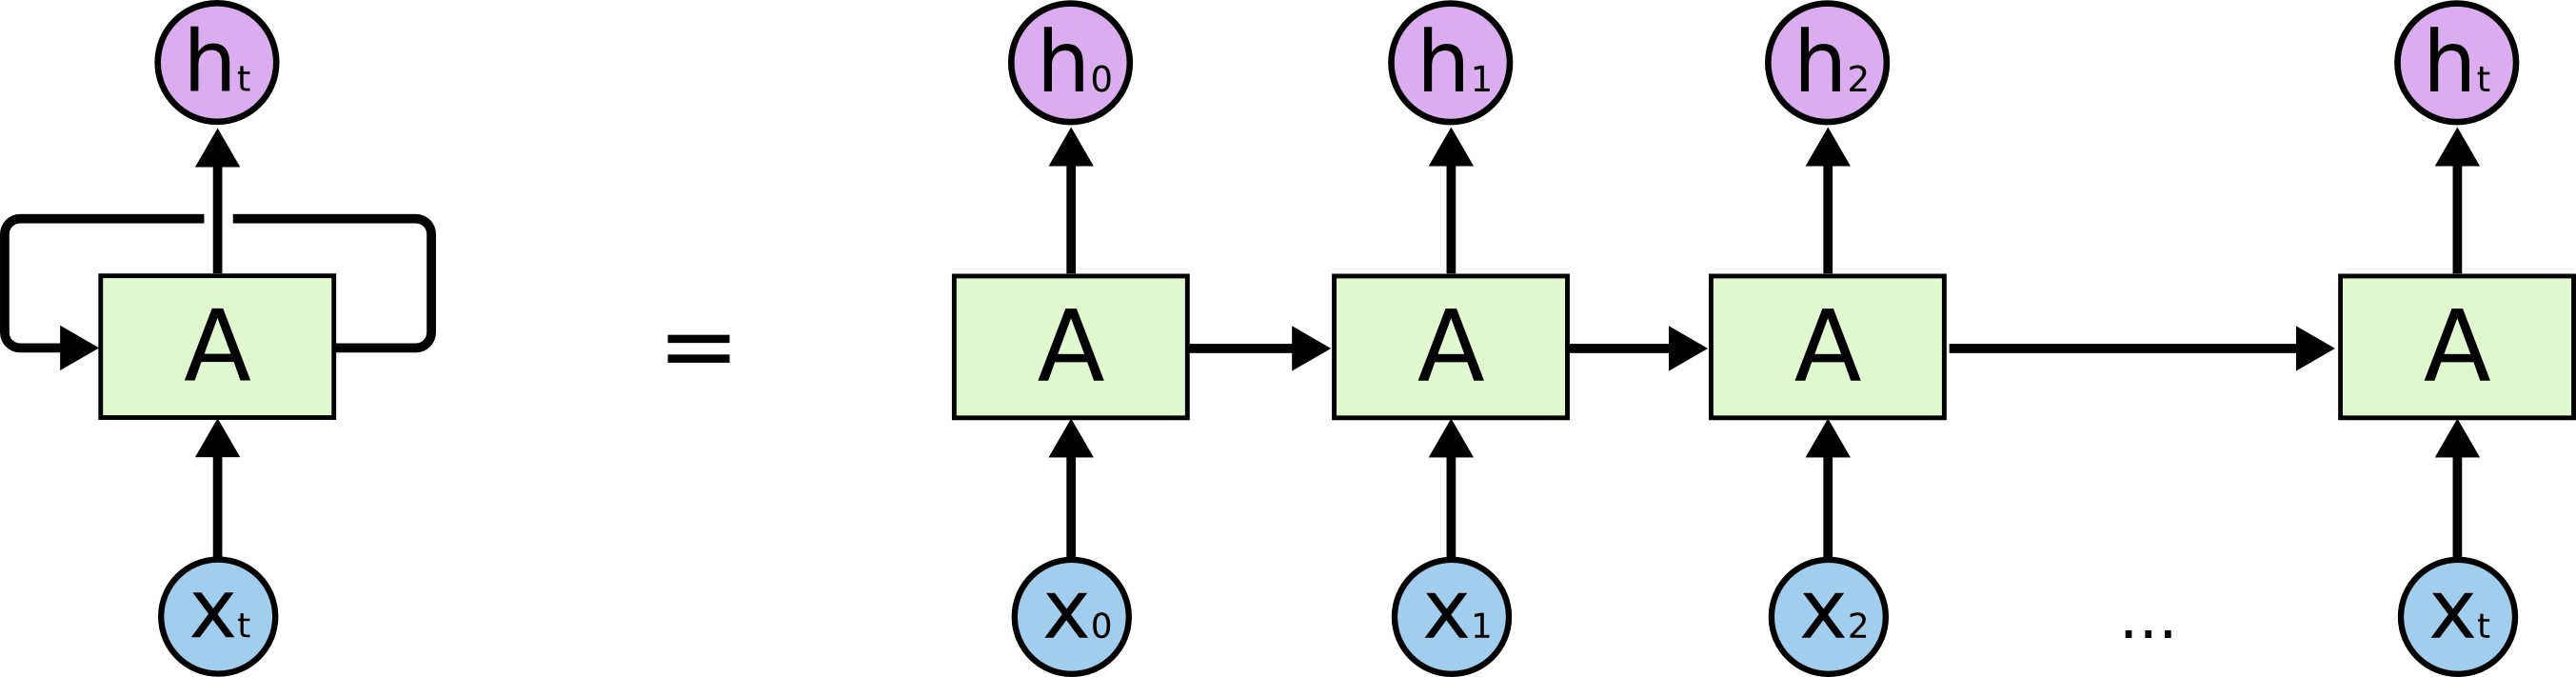
\includegraphics[width=0.5\linewidth]{images/notions/rnns.png}
	%			\caption{Un réseau de neurones récurrent durant les différentes étapes $t$ \citep{rnns_online}}
	
	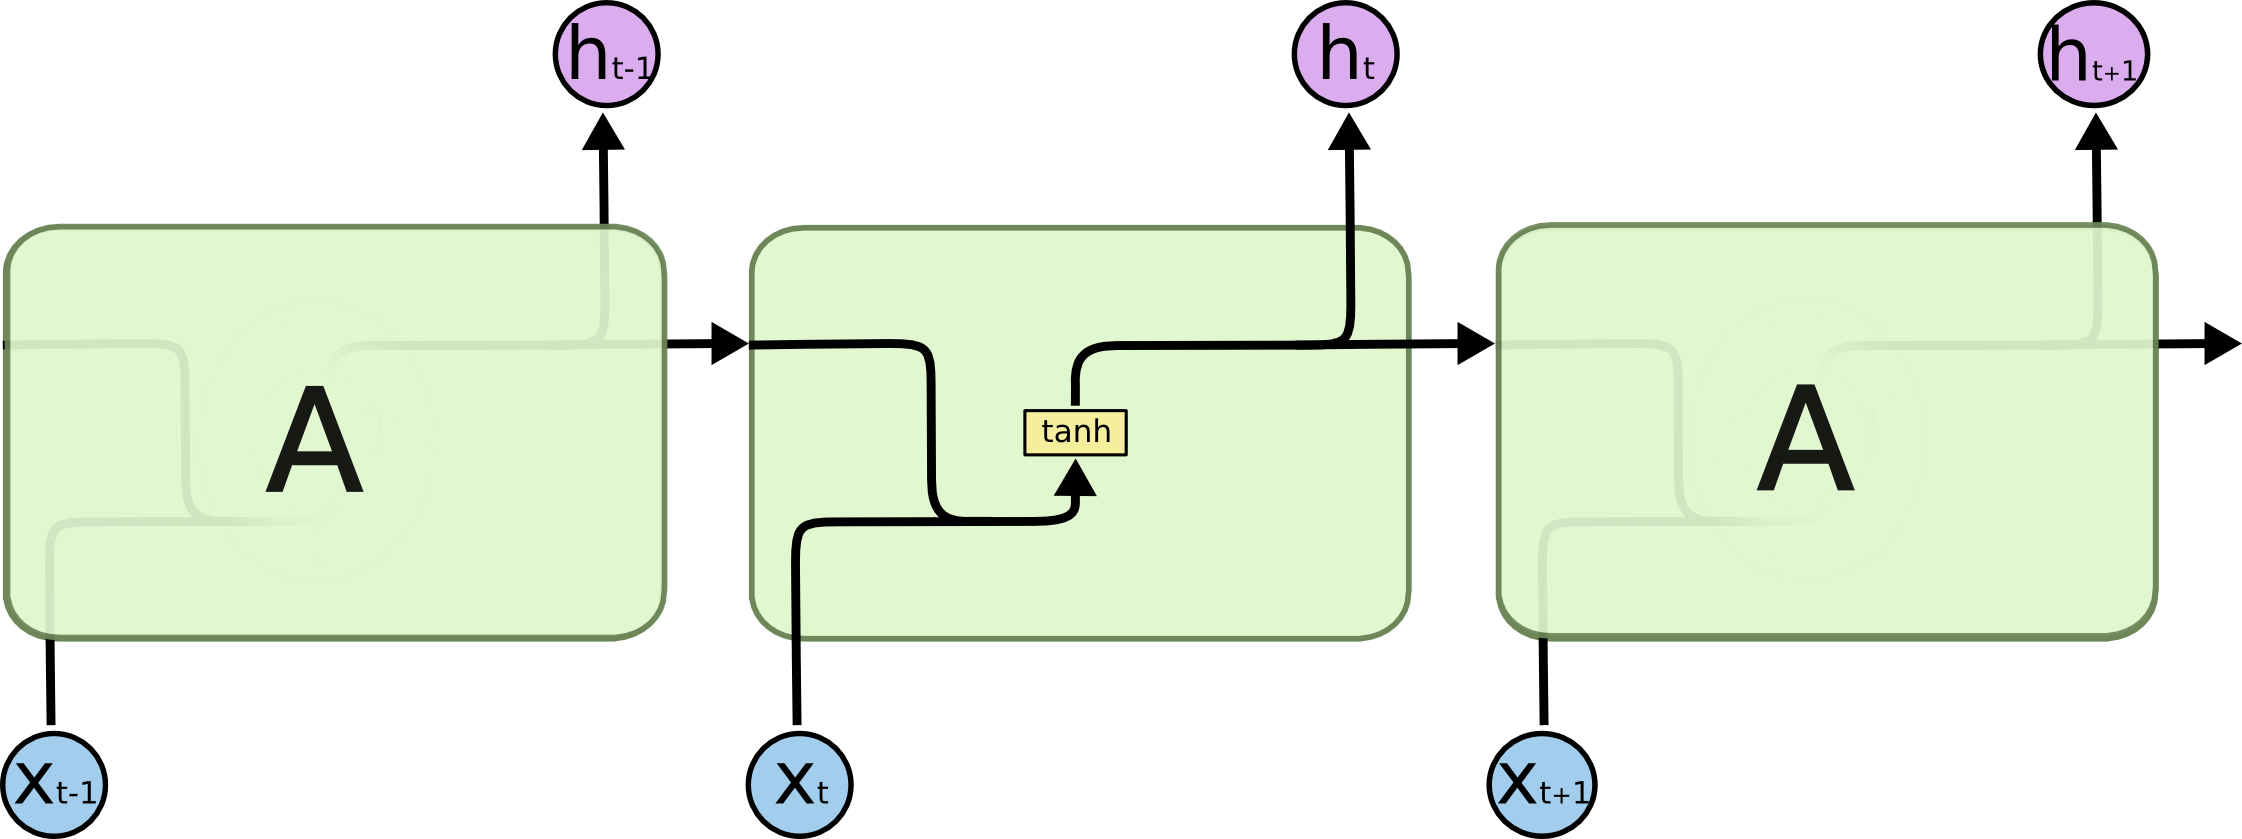
\includegraphics[width=0.5\linewidth]{images/notions/rnns_unrolled_online.png}
	\caption{Architecture interne d'un réseau de neurones récurrent à un instant $t$ \citep{rnns_online}}
\end{figure}
\par 
Un des principaux problèmes que rencontrent les RNNs est celui du \textit{"Vanishing gradient"} traduit par le \textit{"Problème de disparition du gradient"} \citep{vanishing_gradient}. Les relations à long terme entre les séquences ne sont donc pas capturées. Ainsi, pour remédier à ce problème, des architectures de réseaux de neurones dotées d'un module de mémoire ont étés introduites.

\subsubsection*{Réseaux de neurones récurrents à mémoire à court et long terme (LSTM)}
\paragraph{}
Introduite en 1997 dans \citep{lstm_original_paper}, cette architecture de réseaux de neurones récurrents est dotée d'un système de \textit{portes} qui filtrent l'information qui y passe ainsi que d'un état interne de la cellule mémoire d'un réseau LSTM. Les composants d'une cellule LSTM  sont détaillés dans la figure \ref{lstm_architecture} qui suit : 
\begin{figure}[H]
	\centering
	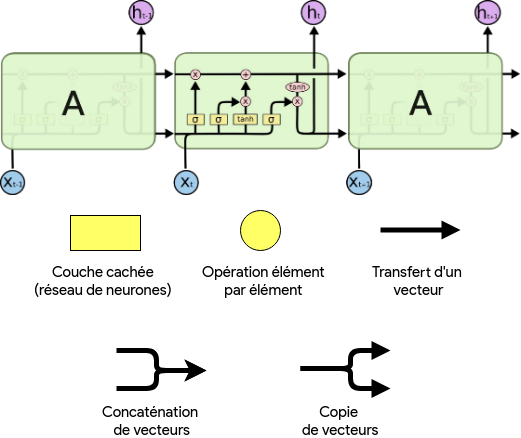
\includegraphics[width=0.5\linewidth]{images/notions/lstm_arch.png}
	\caption{Architecture interne d'une cellule mémoire dans un réseau LSTM \citep{rnns_online}}
	\label{lstm_architecture}
\end{figure}
\begin{itemize}
	\item \textbf{Porte d'entrée (Input gate): } C'est une unité de calcul qui laisse passer certaines informations en entrée en utilisant une fonction d'activation sigmoïde pour pondérer les composants du vecteur d'entrée à une étape $t$ et celles du vecteur d'état interne à l'étape $t-1$ (1: laisser passer, 0: ne pas laisser passer) et ainsi générer un vecteur candidat $\tilde{C}_t$ \citep{lstm_original_paper}.
	\begin{equation}
	\begin{gathered}
	i_t = \sigma(W_i \times [h_{t-1},x_t] + b_i) \\
	\tilde{C}_t = \tanh(W_C \times [h_{t-1},x_t] + b_C)
	\end{gathered}
	\end{equation}
	où : 
	\begin{itemize}
		\item $h_{t-1}$ et $x_t$ sont respectivement le vecteur d'état caché à l'étape $t-1$ et le vecteur de données en entrée à l'étape $t$.
		\item $\sigma$ est la fonction Sigmoïde. 
		\item $i_t$ est appelé le vecteur d'entrée de la cellule LSTM.
		\item $W_i$ est la matrice de poids entre les entrées (plus précieusement, l'état précédent et la nouvelle donnée) et le vecteur d'entrée de la cellule LSTM.
		\item $b_i$ est un vecteur de biais.
		\item $\tilde{C}_t$ est le vecteur d'état interne candidat. 
		\item $W_C$ est la matrice de poids entre le vecteur d'entrée de la cellule LSTM et le vecteur d'état interne candidat.
		\item $b_C$ est un vecteur de biais.
		\item $\tanh$ est la fonction Tangente Hyperbolique. 		
	\end{itemize}
	\item \textbf{Porte d'oubli (Forget gate): } De manière similaire, cette porte permet de spécifier au fur et à mesure de l'apprentissage les informations à oublier, qui sont donc peu importantes \citep{lstm_original_paper,rnn_lstms}.
	\newpage
	\begin{equation}
	\begin{gathered}
	f_t = \sigma(W_f \times [h_{t-1},x_t] + b_f)
	\end{gathered}
	\end{equation}
	
		où : 
	\begin{itemize}
		\item $f_t$ est appelé le vecteur d'oubli de la cellule LSTM.
		\item $W_f$ est la matrice de poids entre les entrées et le vecteur d'oubli de la cellule LSTM.
		\item $b_f$ est un vecteur de biais.		
	\end{itemize}
	\item \textbf{État interne de la cellule (Internal cell's state ): } C'est une sorte de convoyeur qui fait circuler l'information à travers la cellule. Cet état est mis à jour à travers la combinaison des vecteurs $C_{t - 1}$ et $\tilde{C}_t$ filtrés par les portes $f_t$ et $i_t$ \citep{lstm_original_paper}.
	
	\begin{equation}
	\begin{gathered}
	C_t = f_t * C_{t-1} + i_t*\tilde{C}_t
	\end{gathered}
	\end{equation}
	où :
	\begin{itemize}
		\item $C_{t-1}$ est le vecteur d'état interne de la cellule LSTM à l'instant $t-1$.
	\end{itemize}
	\item \textbf{Porte de sortie (Output gate): } Pour renvoyer un résultat comme état caché du réseau, la cellule filtre son vecteur d'état interne $C_t$ et le combine avec la donnée en entrée et l'état du réseau précédent pour ne laisser passer que certaines informations \citep{rnns_online,lstm_original_paper,rnn_lstms}.
	
	\begin{equation}
	\begin{gathered}
	o_t =  \sigma(W_o \times [h_{t-1},x_t] + b_o) \\
	h_t = o_t * \tanh(C_t)
	\end{gathered}
	\end{equation}
	où :
	\begin{itemize}
		\item $o_{t}$ est un vecteur de sortie temporaire de la cellule LSTM à l'instant $t$.
		\item $W_o$ est la matrice de poids entre les entrées et le vecteur de sortie temporaire de la cellule LSTM.
		\item $b_o$ est un vecteur de biais.
			
	\end{itemize}
\end{itemize}

\subsection{Modèles de Markov cachés (Hidden Markov Models HMM)}
\paragraph{}
Informellement, un modèle de Markov caché (HMM) est un outil de représentation pour modéliser la distribution de probabilité d'une séquence d'observations. Il est dit \textit{caché} pour deux raisons. Premièrement, il est supposé qu'une observation $O$ à un instant $t$ (dénotée $O_t$)  est le résultat d'un certain processus (souvent stochastique) dont l'état $S_t$ est caché à l'observateur. Deuxièmement, l'état $S_t$ du processus caché ne dépend uniquement que de son état à l'instant $t-1$. Il est alors dit que ce processus est Markovien ou qu'il satisfait la propriété de Markov \citep{hmm_intro,markov_process}. D'une façon plus intuitive, un HMM  est utilisé pour modéliser un processus dont les observations sont régies par un autre processus qui ne peut pas être directement observé.
\par De façon plus formelle, un HMM est un 5-tuple $<S,V,\Pi,A,B>$ \citep{hmm_formal} où :
\begin{itemize}
	\item $S = \lbrace s_1,...,s_N \rbrace$ est l'ensemble fini des $N$ états du processus sous-jacent.
	\item $V = \lbrace v_1,...,v_M \rbrace$ est l'ensemble des $M$ symboles qui constitue un certain vocabulaire.
	\item $\Pi = \lbrace \pi_i \rbrace$ est une distribution initiale des probabilité d'états tel que $\pi_i$ est la probabilité de se trouver à l'état $i$ à l'instant $t=0$, avec $\sum_{i=1}^{N} \pi_i = 1$ 
	\item $A=\lbrace a_{ij} \rbrace$ est une matrice $N \times N$ dont chaque entrée $a_{ij}$ est la probabilité de transition d'un état $i$ à un état $j$ avec $\sum_{j=1}^{N} a_{ij} = 1$ pour tout $i = 1,...,N$.
	\item $B=\lbrace b_i(v_k)\rbrace$ est l'ensemble des distributions de probabilités d'émission (ou d'observation), donc $b_i(v_k)$ est la probabilité de générer un symbole $v_k$ du vocabulaire étant donné un certain état $i$ avec $\sum_{k=1}^{M} b_{i}(v_k) = 1$ pour tout $i= 1,...,N$. 
	
	\begin{figure}[H]
		\centering
		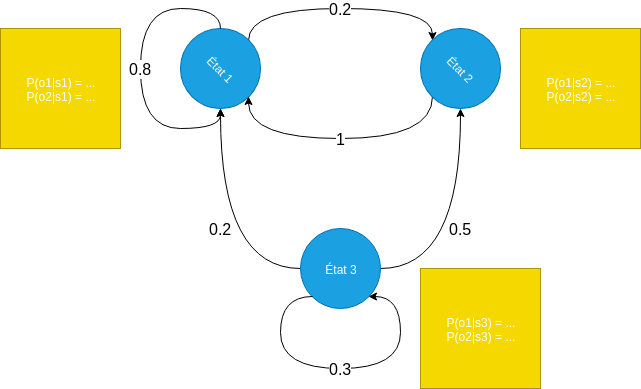
\includegraphics[width=0.65\linewidth]{images/notions/hmm.png}
		\caption{Exemple d'une distribution de probabilités de transitions ainsi qu'une distribution de probabilités d'observations pour un HMM à 3 états et 2 observations}
		\label{hmm_process}
	\end{figure}
\end{itemize}
\paragraph{}
Le but est de trouver la séquence d'états $S_{1:K}$ qui maximise la probabilité \citep{hmm_intro} : 
\begin{equation}
P(Y_{1:K} | O_{1:K}) = P(O_1)P(O_1|S_1)\prod_{t=2}^{K}P(S_t|S_{t-1})P(O_t|S_t) 
\end{equation}
Pour y parvenir d'une manière efficace, un décodeur qui implémente l'algorithme de viterbi peut être utilisé \citep{viterbi,viterbi_hmm}.

\section{Reconnaissance automatique de la parole (ASR)}
\paragraph{}
Le premier module qui compose le système est celui de la reconnaissance automatique de la parole (ASR). Le but d'un tel système (ou sous-système dans notre cas) est de convertir un signal audio correspondant à la locution d'un utilisateur en un texte qui peut être interprété par la machine \citep{asr_definition}. Différentes approches ont été développées au cours des années. Une architecture s'est ensuite dégagée où les systèmes passent par deux phases : la phase d'apprentissage et la phase de reconnaissance. La première consiste à collecter les données qui constituent le corpus d'apprentissage, un ensemble de fichiers audios avec leurs transcriptions en texte et en phonèmes. Le signal est ensuite traité pour en extraire des vecteurs de caractéristiques (ou attributs). La suite de l'apprentissage consiste à initialiser le HMM, lui passer les vecteurs précédemment extraits puis l'enregistrer pour la phase suivante qui est la reconnaissance. Dans la deuxième phase, le signal audio passe par le même procédé d'extraction des attributs, en utilisant un algorithme de décodage approprié \citep{viterbi_hmm}, puis la séquence d'observations passe par le HMM et la meilleure séquence de mots est sélectionnée \citep{speech_reco_Yu2015}.
\par Une architecture assez générale s'est dégagée. Quatre modules sont impliqués dans le processus de la reconnaissance de la parole; nous les citerons dans les sections qui suivent en énumérant les modèles utilisés dans chacun.

\begin{figure}[H]
	\centering
	\label{ASRSchema}
	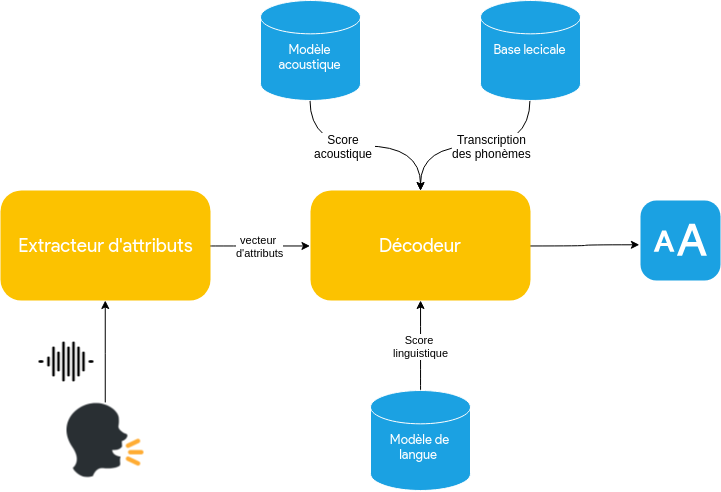
\includegraphics[width=0.70\linewidth]{images/ASR/schema.png}
	\caption{Architecture d'un système de reconnaissance de la parole \citep{speech_reco_Yu2015}}
\end{figure}

\subsection{Acquisition du signal et extraction d'attributs}
\paragraph{}
L'étape consiste à extraire une séquence de vecteurs caractéristiques à partir du signal audio, fournissant une représentation compacte de ce dernier. Le processus démarre par la segmentation du signal en \textit{trames}. Une transformation de fourrier est ensuite appliquée pour engendrer un spectre de magnitude qui sera ensuite passé à un module de transformation en spectre de Mel (Mel-Spectrum) qui est une sorte de changement d'échelle. Finalement, une transformation inverse de fourrier est appliquée pour engendrer le Mel-Cpestrum qui est le vecteur d'attributs que nous recherchions \citep{asr_extraction}. Un tel processus peut utiliser plusieurs techniques pour la mise à l'échelle: MFCC (Mel-frequency cepstrum) \citep{MFCC}, LPC (Linear Predictive coding) \citep{LSP} et RASTA (RelAtive SpecTrAl) \citep{RASTA}, chacune possédant ses avantages et ses inconvénients.
\subsection{Modélisation acoustique et modélisation du lexique}
\paragraph{}
C'est le c\oe{}ur du système de reconnaissance. Le but est de construire un modèle permettant d'identifier une séquence de phonèmes à partir d'une séquence d'observations de vecteurs d'attributs. Ceci peut être fait en utilisant un modèle HMM et en disposant d'un corpus de fichiers audio accompagnés de leurs transcriptions en phonèmes et en texte \citep{hmm_acoustic_model,hmm_formal}, ou bien un réseau de neurones profonds \citep{speech_reco_Yu2015}, ou encore une hybridation de ces derniers \citep{dnn-hmm_acoustic_model}. Le modèle acoustique procède après la reconnaissance de la séquence de phonèmes au décodage de ce dernier. Ceci est effectué en utilisant un dictionnaire linguistique qui transcrit chaque mot du vocabulaire en phonèmes qui le constituent. Ceci peut conduire à un cas d'ambiguïté où plusieurs mots peuvent avoir la même transcription phonétique (ou bien aucun mot ne correspond à cette séquence). Pour lever cette ambiguïté, un modèle de langue est nécessaire pour décider quelle est la séquence de mots la plus probable qui coïncide avec la séquence de phonèmes observée.  
\subsection{Modélisation de la langue}
\paragraph{}
Cette étape consiste à modéliser les aspects linguistiques de la langue que le système essaye de traiter. Souvent ces aspects sont spécifiques au domaine d'application afin de restreindre l'espace de recherche des mots reconnaissables par le système, puis de déterminer la séquence de mots en sortie la plus plausible. Les modèles utilisés sont basés soit sur des grammaires à contexte libre dans le cas où les séquences de mots reconnaissables sont peu variées et peuvent être modélisées par le biais de règles de la langue \citep{LM_grammar}; ou alors dans un cadre plus récent, sur des modèles probabilistes basés sur les N-grammes.
\par
\label{n-grams}
Très souvent, quand il est nécessaire de traiter un ensemble de mots, phrases ou bien toute entité atomique qui constitue une séquence, il est intéressant de pouvoir assigner une probabilité de vraisemblance à une séquence donnée (par exemple une séquence de mots). 
\par Dans un contexte textuel, un N-gramme est une suite de N mots \footnote{Dans certains cas, un N-gramme peut être aussi une suite de lettres/caractères} consécutifs qui forment une sous-chaîne $S'$ d'une chaîne de caractères $S$. Un exemple d'un ensemble de bi-grammes (2-grammes) pour la phrase "Ouvre le fichier \textit{home}" serait donc : (Ouvre,le), (le,fichier), (fichier,\textit{home}).
\par 
Ainsi, en disposant d'un corpus de textes assez large et diversifié et d'une méthode de comptage efficace, il serait possible de calculer la vraisemblance d'apparition d'un mot $w$ après une certaine séquence de mots $t$ sous forme d'une probabilité $P$ \citep{nlp_ngrams}.
\begin{equation}
P(w|t) = \frac{Comptage(t,w)}{Comptage(t)}
\end{equation}
\par
Disposant d'un volume de données textuelles assez conséquent, l'utilisation de modèles basés sur les N-grammes a prouvé son utilité \citep{nlp_ngrams,speech_reco_Yu2015,LM_n-grams} .


\section{Compréhension du langage naturel}
\paragraph{}
\label{nlu_chap2}
Après avoir obtenu la requête de l'utilisateur, le module qui prend le relais est celui de la compréhension du langage naturel (Natural Langage Understanding, NLU). Ce domaine fait partie du traitement automatique du langage naturel (Natural Langage Processing, NLP). Il se focalise principalement sur les tâches qui traitent le niveau sémantique, voire même pragmatique, de la langue tel que la classification de texte, l'analyse de sentiments ou encore le traitement automatiques des e-mails. Dans le contexte d'un SPA, le but final d'un module de compréhension du langage naturel est de construire une représentation sémantique de la requête de l'utilisateur. Étant donné une telle requête préalablement transformée en texte brut dans un langage naturel, le module essayera d'en extraire une information primordiale qui est l'intention du locuteur.

\subsection{L'intention}
\paragraph{}
L'intention est un élément clé dans notre travail. Nous allons donc la définir et expliquer pourquoi elle a été choisie comme abstraction sémantique d'une requête d'un utilisateur. \par

Une intention (ou intent en anglais) est une représentation sémantique d'un but ou d'un sous-but de l'utilisateur. Plusieurs requêtes de l'utilisateur peuvent avoir le même intent, ce qui rend l'utilisation d'une telle représentation essentielle pour que la machine puisse mieux comprendre l'utilisateur. La motivation vient du fait que la machine ne peut pas comprendre une requête formulée dans un langage non-formel. Il a fallu trouver un moyen de communication universel entre la machine et l'utilisateur de telle sorte que l'un puisse "comprendre" l'autre . L'intermédiaire entre ces deux parties est un traducteur bidirectionnel d'une requête en langage naturel vers une requête dans un langage formel et inversement. 
\par Le choix de l'intention doit être minutieusement étudié au préalable pour ne pas trop subdiviser un type d'intention, tout en gardant un certain degré de spécificité. À titre d'exemple, si deux intentions $Ouvrir\_fichier$ et $Ouvrir\_document$ existent, on retrouve ici une répétition de l'information $fichier$ qui est aussi un $document$. Dans ce cas il suffit d'éliminer un synonyme pour ne garder qu'un seul cas d'intention. \par
Un autre cas est celui du sur-découpage d'intentions déjà assez semblable, $Ouvrir\_fichier$ et $Ouvrir\_Repertoire$ peuvent être regroupés en une seule intention $Ouvrir\_Entite$. Bien-sur ces choix sont purement conceptuels et dépendent fortement du problème traité par le système. Choisir une représentation à la place d'une autre est lié à la nature de la tâche que le module doit accomplir \citep{intent_classification,intent_slots}.
\subsection{Classification d'intentions}
\paragraph{}
La classification d'intentions à partir d'un texte est une tâche réalisable avec des techniques récentes d'apprentissage automatique, plus précisément en utilisant des modèles basés sur les réseaux de neurones récurrents à "mémoire à court et long terme" (LSTM) (voir la section \ref{lstm_architecture}). Dans \citep{intent_classification} et \citep{intent_slots} deux architectures qui ont fait leurs preuves sont présentées. Dans le premier travail, les auteurs ont utilisé une architecture BiLSTM (LSTM Bidirectionnel) pour capturer les contextes droit et gauche d'un mot donné \citep{blstm}. Le dernier état caché retourné par la cellule LSTM est ensuite utilisé pour la classification. Une couche d'attention est ajoutée \citep{attention_mechanism} pour permettre au modèle de se focaliser sur certaines parties du texte en entrée. La deuxième architecture est un peu plus simple. En effet, elle utilise des cellules LSTM basiques avec une couche de classification sur le dernier état. L'avantage par rapport à la première architecture est le temps d'apprentissage assez réduit au détriment d'une erreur de classification plus accrue mais toujours dans les normes.
\begin{figure}[H]
	\centering
	\label{LSTM_intent}
	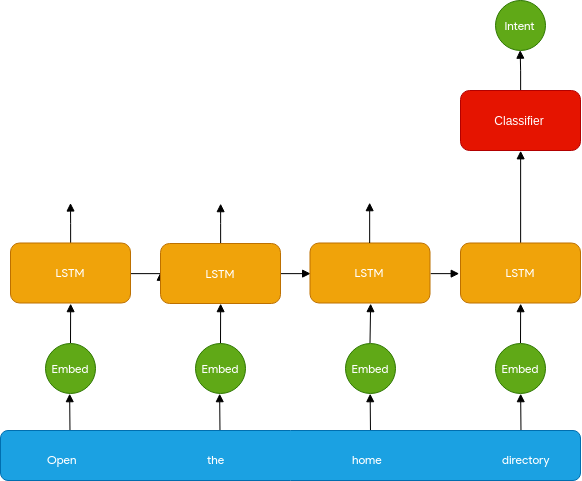
\includegraphics[width=0.65\linewidth]{images/NLU/intent_classification.png}
	\caption{Architecture de base d'un classificateur d'intentions (intents) \citep{intent_classification}}
\end{figure}
\subsection{Extraction d'entités}
\paragraph{}
Déterminer l'intention d'un utilisateur ne s'arrête pas au stade de l'identification de l'\textit{intent}. En effet, pour mieux représenter l'information récoltée depuis la requête, il faut en extraire des entités (nommées ou spécifiques du domaine) qui seront des arguments de l'intent identifié. Cette tâche consiste donc, pour une intention $I$ donné, à extraire les arguments $Args$ qui lui sont appropriés depuis le texte de la requête. Plusieurs approches sont possibles. Dans \citep{intent_slots} les auteurs ont attaqué le problème comme étant la traduction d'une séquence de mots en entrée en une séquence d'entités en sortie; le schéma suivant explicite le processus :
\begin{figure}[H]
	\centering
	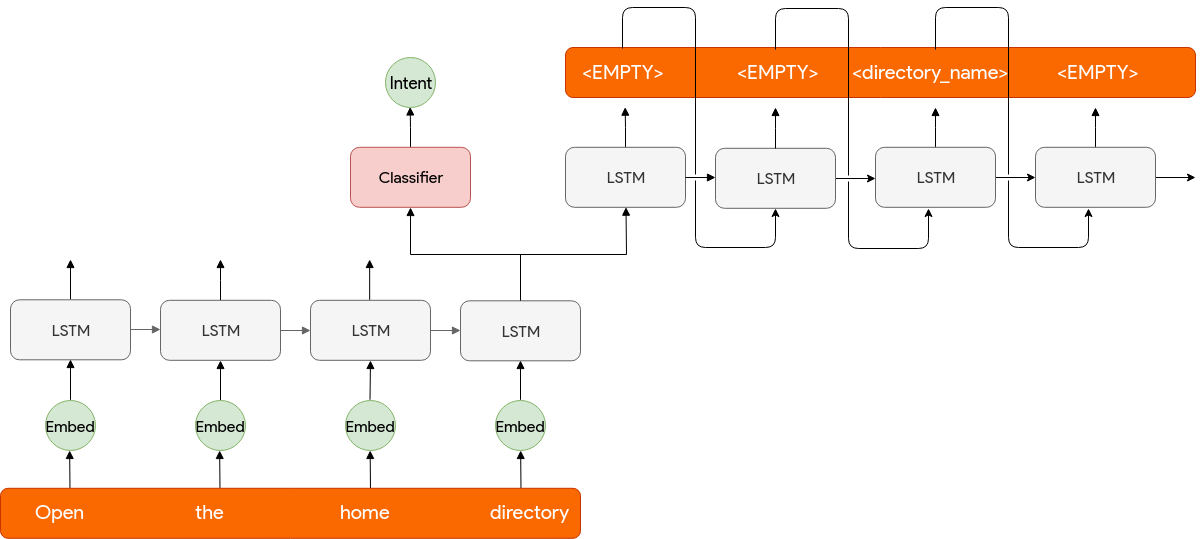
\includegraphics[width=0.85\linewidth]{images/NLU/seq2seq.png}
	\caption{Architecture de base d'un classificateur d'intentions doublé d'un extracteur d'entités \citep{intent_slots}}
	\label{fig:lstmslots}
\end{figure} 
\subsection{Analyse sémantique}
\paragraph{}
Disposant des deux modèles précédemment cités, le module NLU peut construire une représentation sémantique adéquate qui va être transmise au module suivant qui sera le gestionnaire du dialogue. L'avantage d'avoir en sortie une structure sémantique universelle est la non-dépendance par rapport à la langue de l'utilisateur. En effet, le système pourra encore fonctionner si une correspondance entre la nouvelle langue et le format choisi pour la représentation sémantique peut être trouvée. Le module donnera donc en sortie une trame sémantique (Semantic frame) qui comprendra les informations préalablement extraites, à savoir l'intention et les arguments (slots) qui lui sont propres \citep{intent_classification,intent_slots,semantic_frame}.
\begin{figure}[H]
	\centering
	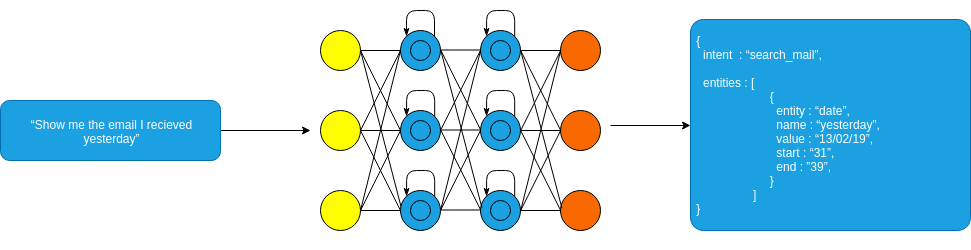
\includegraphics[width=0.80\linewidth]{images/NLU/semantic_frames.png}
	\caption{Exemple d'une trame sémantique pour une requête donnée}
	\label{fig:semanticFrame}
\end{figure} 
\section{Gestion du dialogue}
\paragraph{}
La compréhension du langage naturel permet de transformer un texte en une représentation sémantique. Afin qu'un système puisse réaliser un dialogue aussi anthropomorphe que possible, il doit décider, à partir des représentations sémantiques reçues au cours du dialogue, quelle action prendre à chaque étape de la conversation. Cette action est transmise au générateur du langage naturel (voir \ref{NLG}) pour afficher un résultat à l'utilisateur. Généralement, deux principaux modules sont présents dans les systèmes de gestion de dialogue:
\begin{itemize}
	\item Un module qui met à jour l'état du gestionnaire de dialogue: le traqueur d'état.
	\item Un module qui détermine la politique d'action du gestionnaire de dialogue.
\end{itemize}

\begin{figure}[H]
	\centering
	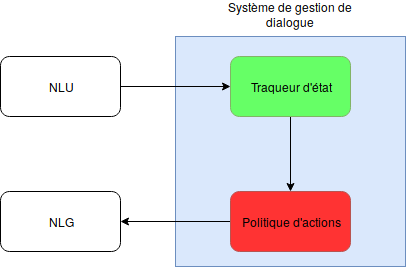
\includegraphics[width=.7\linewidth]{images/DM/DMGeneral.png} 
	\caption{Schéma général d'un gestionnaire de dialogue} 
\end{figure}
\par Ainsi, le gestionnaire de dialogue passe d'un état à un autre après chaque interaction avec l'utilisateur. Le problème à résoudre est donc de trouver la meilleure action à prendre en étant dans un état donné.
%\subsection{Processus de décision Markovien (MDP)}
\subsection{Modélisation}\label{MDP}
\paragraph{}Pour résoudre ce problème, un gestionnaire de dialogue peut être modélisé par un processus de décision Markovien (Markovian Decision Process, MDP) \citep{Bel1957}. Ce dernier est modélisé par un 4-tuple ($S,A,P,R$):
\begin{itemize}
	\item $S$: ensemble des états du système.
	\item $A$: ensemble des actions du système.
	\item $P$: distribution de probabilités de transitions entre états sachant l'action prise. $P(s'/s,a)$ est la probabilité de passer à l'état $s'$ sachant qu'on était à l'état $s$ après avoir réalisé l'action $a$.
	\item $R$: est la récompense reçue immédiatement après avoir changé l'état avec une action donnée. $R(s'/s,a)$ est la récompense reçue après être passé à l'état $s'$ sachant que le système était à l'état $s$ après avoir réalisé l'action $a$.
\end{itemize}
Un MDP, à tout instant $t$, est dans un état $s$. Dans notre cas c'est l'état du gestionnaire de dialogue. Il peut prendre une action $a$ afin de passer à un nouvel état $s'$. De ce fait, il reçoit une récompense qui ,dans notre cas, est une mesure sur les performances du système de dialogue. Le but est de maximiser les récompenses reçues.

\begin{figure}[H]
	\centering
	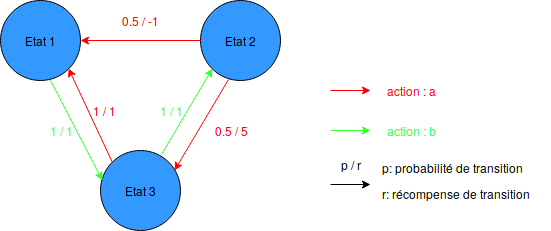
\includegraphics[width=.95\linewidth]{images/DM/MDP.png} 
	\caption{Schéma représentant les transitions entre états dans un MDP} 
\end{figure}


\subsection{État du gestionnaire de dialogue}\label{trame}
\paragraph{}
L'état d'un système de dialogue est une représentation sémantique qui contient des informations sur le but final de l'utilisateur ainsi que l'historique de la conversation. La représentation souvent utilisée dans les systèmes de dialogue est celle de la trame sémantique \citep{Chen2017}. Cette structure contient des emplacements à remplir dans un domaine donné. La figure \ref{SFrame} illustre un exemple de trame sémantique.\newline
\begin{figure}[H]
	\centering
	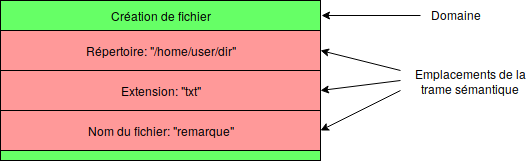
\includegraphics[width=.7\linewidth]{images/DM/SFrame.png} 
	\caption{Schéma représentant une trame sémantique avec comme domaine: création de fichier} 
	\label{SFrame}
\end{figure}


À l'arrivée d'une nouvelle information, un module dédié met à jour l'état du gestionnaire de dialogue. Comme l'action du système de dialogue est décidée à partir de son état, cette tâche est donc essentielle au bon fonctionnement du système. Plusieurs méthodes ont été proposées pour gérer le suivi de l'état du gestionnaire de dialogue \citep{Williams2007}.
\subsubsection{Suivi de l'état du gestionnaire de dialogue avec une base de règles}\label{suivi}
\paragraph{}
La méthode traditionnelle utilisée consiste à écrire manuellement les règles à suivre lors de l'arrivé d'une nouvelle information pour mettre à jour l'état \citep{Goddeau1996}. Cependant, les bases de règles sont très susceptibles à faire des erreurs \citep{Chen2017} car elles sont peu robustes face aux incertitudes.


\begin{figure}[H]
	\centering
	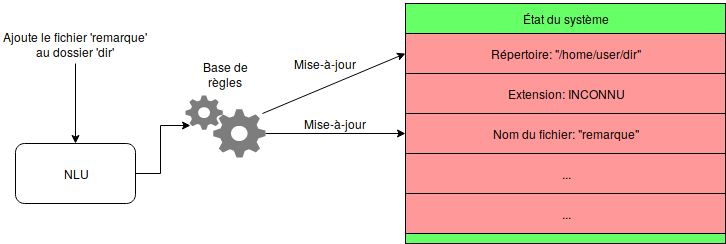
\includegraphics[width=.7\linewidth]{images/DM/RuleBasedUpdate.png} 
	\caption{Schéma représentant la mise-à-jour de l'état du gestionnaire de dialogue par un système basé règles} 
\end{figure}

\subsubsection{Suivi de l'état du gestionnaire de dialogue avec des méthodes statistiques}

Le suivi dans ce cas se fait en gardant une distribution de probabilités sur l'état du système, ce qui nécessite une nouvelle modélisation non déterministe du problème. Les processus de décision markoviens partiellement observables (Partially Observable Markov Decision Process POMDP) \citep{Young2010} sont une variante des MDP capable de répondre à ce besoin que nous introduirons par la suite. Dans ce cas, le système garde une distribution de probabilités sur les valeurs possibles des différents emplacements de la trame sémantique.

\begin{figure}[H]
	\centering
	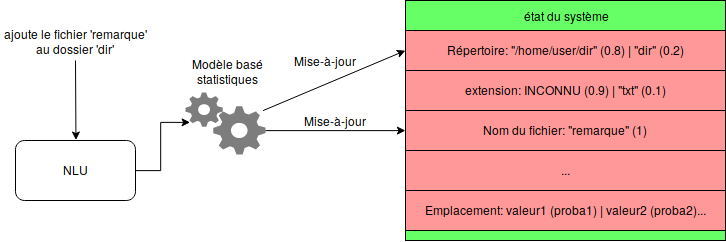
\includegraphics[width=.7\linewidth]{images/DM/StatBasedUpdate.png} 
	\caption{Schéma représentant la mise-à-jour de l'état du gestionnaire de dialogue par un système basé statistiques} 
\end{figure}

\paragraph{Processus de décision markovien partiellement observable (POMDP)}
Comme dans les processus de décision markoviens, un POMDP \citep{Astrom1965} passe d'un état à un autre en prenant une des actions possibles. Cependant, un POMDP ne connait pas l'état exact dans lequel le système se trouve à un instant $t$. Il reçoit par contre une observation qui est, dans notre cas, l'action de l'utilisateur, à partir de laquelle il peut estimer une distribution de probabilités sur l'état actuel. Pour résumer, un POMDP est un 6-tuple ($S,A,P,R,M,O$) où:
\begin{itemize}
	\item Les 4 premiers composants sont les mêmes que ceux d'un MDP (voir \ref{MDP}).
	\item $M$: l'ensemble des observations.
	\item $O$: la distribution de probabilités sur les observations $o$ en connaissant l'état $s$ et l'action $a$ prise pour y arriver. $O(o|s,a)$ est la probabilité d'observer $o$ sachant que le système se trouve à l'état $s$ et qu'il a pris l'action $a$ pour y arriver.
\end{itemize}

\begin{figure}[H]
	\centering
	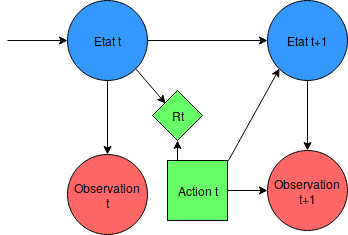
\includegraphics[width=.5\linewidth]{images/DM/POMDP.png} 
	\caption{Diagramme d'influence dans un POMDP} 
\end{figure}

\subsubsection{Suivi de l'état du gestionnaire de dialogue avec réseaux de neurones profonds}
\paragraph{}
Récemment, des approches utilisant les réseaux de neurones profonds (voir \ref{part2DNN}) ont fait leur apparition. En effet, l'utilisation des architectures profondes permet de capter des relations complexes entre les caractéristiques d'un dialogue et, ainsi, mieux estimer l'état du système. Le réseau de neurones estime les probabilités de toutes les valeurs possibles d'un emplacement de la trame sémantique \citep{Henderson2013}. En conséquence, il peut être utilisé comme modèle de suivi d'état pour un processus partiellement observable.

\subsection{Politique de gestion de dialogue}
\paragraph{}
La première partie est dédiée au module qui suit l'état du système de dialogue. Dans cette partie, nous allons présenter des approches proposées afin d'arriver au but du MDP, c'est à dire quelles actions prendre pour maximiser la somme des récompenses obtenues.
\subsubsection{Gestion de dialogue avec une base de règles}
\paragraph{}
Les premières approches utilisaient des systèmes de règles destinés à un domaine bien spécifique. Elles étaient déployées dans plusieurs domaines d'application pour leur simplicité. Cependant, le travail manuel nécessaire reste difficile à faire et, généralement, n'aboutit pas à des résultats flexibles qui peuvent suivre le flux du dialogue convenablement \citep{Lee2010}.
\subsubsection{Gestion de dialogue par apprentissage}
\paragraph{}
La résolution d'un MDP revient à trouver une estimation de la fonction de récompense afin de pouvoir choisir la meilleure action. La majorité des approches récentes utilise l'apprentissage par renforcement dans le but d'estimer la récompense obtenue par une action et un état donnés. Cette préférence par rapport aux approches supervisées revient à la difficulté de produire des corpus de dialogues \citep{Henderson2008}, encore moins des corpus annotés avec les récompenses à chaque transition. Néanmoins, il existe des approches de bout en bout qui exploitent des architectures avec réseaux de neurones profonds et traitent le problème comme Seq2Seq\footnote{Les modèles Seq2Seq sont des architectures de réseaux de neurones profonds qui prennent en entrée une séquence et produisent en sortie une autre séquence en utilisant les réseaux de neurones récurents (RNN).} afin de produire directement une sortie à partir des informations reçues de l'utilisateur \citep{Wen2017,Serban2016}.


\begin{figure}[H]
	\centering
	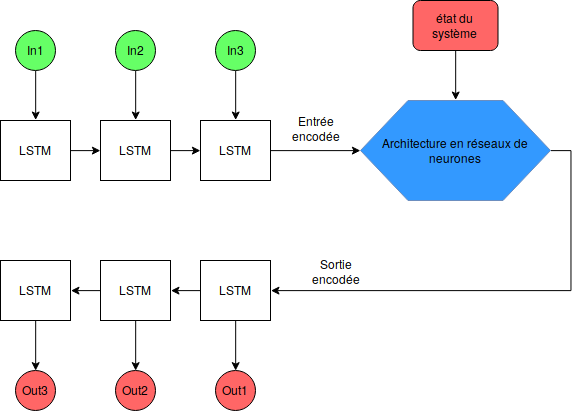
\includegraphics[width=.7\linewidth]{images/DM/DMSeq2Seq.png} 
	\caption{Schéma de gestion de dialogue de bout en bout avec architecture Seq2Seq} 
\end{figure}
\subsubsection{Apprentissage par renforcement} \label{reinf_learning}
\paragraph{}
L'apprentissage par renforcement est une approche qui a pour but d'estimer une politique d'actions à prendre dans un environnement donné. Cette politique doit maximiser une mesure d'évaluation qui est sous forme de récompenses obtenues après chaque action \citep{Weisz2018}. L'environnement est souvent modélisé comme un MDP, ou éventuellement POMDP. L'agent d'apprentissage passe donc d'un état à un autre en prenant des actions dans cet environnement. L'apprentissage se fait dans ce cas en apprenant par l'expérience de l'agent, à savoir les récompenses obtenues par les actions prises dans des états donnés. Il peut ainsi estimer la fonction de récompense pour pouvoir faire le choix d'actions optimales. 

\begin{figure}[H]
	\centering
	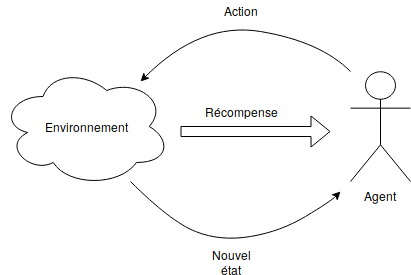
\includegraphics[width=.5\linewidth]{images/DM/RLSchema.png} 
	\caption{Schéma d'interaction agent-environnement dans l'apprentissage par renforcement} 
\end{figure}
Il existe plusieurs méthodes que l'agent peut utiliser pour estimer la fonction de récompense \citep{Dimitri2012}, notamment Deep Q Learning (DQN) \citep{Mnih2015} qui utilise les réseaux de neurones profonds pour trouver une approximation à cette fonction. Dans cette approche, à chaque fois que l'agent prend une action, il compare la récompense reçue avec celle estimée par le réseau de neurones, et applique ensuite l'algorithme de rétro-propagation pour corriger les erreurs du réseau. 

\paragraph{}\label{usersim}
Le système de dialogue est modélisé par un MDP. Seulement, ce dernier inclut l'utilisateur comme partie de l'environnement. Par conséquent, pour appliquer l'apprentissage par renforcement, il est nécessaire qu'un utilisateur communique avec le système pour qu'il apprenne. D'où la nécessité d'utiliser un \textbf{simulateur d'utilisateur} qui est un programme capable de se comporter comme un humain interagissant avec un système de dialogue. Le simulateur doit pouvoir estimer la satisfaction de l'utilisateur après une interaction. En d'autres termes, il doit comporter une fonction de récompense. Il existe plusieurs méthodes pour créer un simulateur d'utilisateur:
\begin{itemize}
	\item Les simulateurs d'utilisateur basés règles: dans ce cas une liste de règles est écrite manuellement et le simulateur doit les suivre pour communiquer avec le système \citep{Schatzmann2007}.
	\item Les simulateurs d'utilisateur basés n-grammes: ils traitent un dialogue comme une séquence d'actions en prenant les n-1 actions précédentes pour estimer l'action la plus probable que peut prendre le simulateur à partir des statistiques tirées d'un corpus de dialogues \citep{Georgila2005}.
	\item Les simulateurs d'utilisateur basés HMM: les états du modèle sont les états du système et les observations sont ses actions. Ainsi un HMM peut estimer l'état le plus probable du système pour prendre une action. Il existe d'autres variantes, IHMM et IOHMM, qui incluent les probabilités conditionnelles des actions de l'utilisateur sachant l'état du système ou l'action du système directement dans le modèle HMM \citep{Cuayhuitl2005}.
	\item Les simulateurs d'utilisateur avec apprentissage par renforcement: Comme le gestionnaire de dialogue, le simulateur apprend par renforcement au même temps. Dans ce cas la fonction de récompense pour les deux agents peut être apprise à partir des dialogues humain-humain \citep{Chandramohan2011}.
\end{itemize}







\section{Génération du langage naturel (Natural Language Generation, NLG)}\label{NLG}
\paragraph{}
Le domaine de la génération automatique du langage naturel est l'un des domaines dont les limites sont difficiles à définir \citep{evans2002}. Il est vrai que la sortie d'un tel système est clairement du texte. Cependant, l'ambiguïté se trouve dans ses entrées, c'est-à-dire, sur quoi se basera le système pour générer le texte. D'après \citep{Reiter:1997}, la génération du langage naturel est décrite comme étant le sous domaine de l'intelligence artificielle qui traite la construction des systèmes de génération de texte à partir d'une représentation non-linguistique de l'information. Celle-ci peut être une représentation sémantique, des données numériques, une base de connaissances ou même des données visuelles (images ou vidéos). Ceci dit, d'autres travaux, comme \citep{Labbé2012}, utilisent les mêmes techniques pour des entrées linguistiques. Enfin, la génération du langage naturel peut être très proche de la gestion de dialogue \citep{Dethlefs2014}. En effet, le texte généré doit prendre en compte l'historique de la conversation et le contexte de l'utilisateur.\newline
Il existe six tâches trouvées fréquemment dans les systèmes de génération de texte \citep{Reiter:1997}; nous les présentons dans cette section.

\subsection{Détermination du contenu}
\paragraph{}
Cette partie consiste à sélectionner les informations de l'entrée dont le système veut transmettre leur contenu sous forme de texte naturel à l'utilisateur. En effet, les données en entrée peuvent contenir plus d'informations que ce que l'on désire communiquer \citep{Yu:2007}. De plus, le choix de l'information peut aussi dépendre de l'utilisateur et de ses connaissances \citep{Dethlefs2014}. Ceci requiert de mettre au point un système qui détecte les informations pertinentes à l'utilisateur.
\subsection{Structuration de texte}
\paragraph{}
Après la détermination du contenu, le système doit ordonner les informations à transmettre. Ceci dépend grandement du domaine d'application qui peut exiger des contraintes d'ordre temporel ou de préférence par importance des idées. Les informations à transmettre en elles-mêmes sont souvent reliées par sens, ce qui implique une certaine structuration de texte à respecter.
\subsection{Agrégation de phrases}
\paragraph{}
Certaines informations peuvent être transmises dans une même phrase. Cette partie introduit des notions de la linguistique afin que le texte généré soit plus lisible et éviter les répétitions. Un exemple de cela peut être la description de la météo à Alger au cours de la matinée:
\begin{itemize}
	\item Il va faire 16\textdegree{} à Alger à 7h.
	\item Il va faire 17\textdegree{} à Alger à 8h.
	\item Il va faire 18\textdegree{} à Alger à 9h.
	\item Il va faire 18\textdegree{} à Alger à 10h.
\end{itemize}
Ceci peut être agrégé en un texte plus compacte: "La température moyenne à Alger sera de 17.25\textdegree entre 7h et 10h."

\subsection{Lexicalisation}
\paragraph{}Le système choisit les mots et les expressions à utiliser pour communiquer le contenu des phrases sélectionnées. La difficulté de cette tâche revient à l'existence de plusieurs manières d'exprimer la même idée. Cependant, certains mots ou expressions sont plus appropriés en certaines situations que d'autres. En effet, "inscrire un but" est une façon inadéquate d'exprimer "un but contre son camp" \citep{Gatt2018}.

\subsection{Génération d'expressions référentielles (REG)}
\paragraph{}Cette partie du système se focalise sur la génération d'expressions référentielles qui peuvent être entre autres: des noms propres, groupes nominaux ou pronoms et ceci a pour but d'identifier les entités du domaine. Cette tâche semble être très proche de la lexicalisation dans le sens où elle aussi a pour but de choisir les mots et les expressions; elle s'avère néanmoins plus délicate dû à la difficulté de confier suffisamment d'information sur l'entité afin de la différencier des autres \citep{Reiter:1997}. Le système doit faire un choix de l'expression référentielle en se basant sur plusieurs facteurs. Par exemple "Mohammed", "Le professeur" ou "Il" faisant référence à la même personne, le choix entre eux dépend de comment l'entité a été mentionnée auparavant, si elle l'a été, et des détails qui l'ont accompagnée. 

\subsection{Réalisation linguistique}
\paragraph{}
La dernière tâche consiste à combiner les mots et expressions sélectionnés pour construire une phrase linguistiquement correcte. Ceci requiert l'utilisation des bonnes formes morphologiques des mots, les ordonner, et éventuellement  l'addition de certains mots du langage afin de réaliser une structure de phrase grammaticalement et sémantiquement correcte. Plusieurs méthodes ont été proposées, principalement les méthodes basées sur des règles manuellement construites (modèles de phrases, systèmes basés grammaires) et des approches statistiques \citep{Gatt2018}.
\paragraph{Modèles de phrases:} La réalisation se fait en utilisant des modèles de phrases prédéfinis. Il suffit de remplacer des espaces réservés par certaines entrées du système. Par exemple, une application dans un contexte météorologique pourrait utiliser le modèle suivant: “la température à [ville] atteint [température]\textdegree{} le [date]”.
\par Cette méthode est utilisée lorsque les variations des sorties de l'application sont minimales. Son utilisation a l'avantage et l'inconvénient d'être rigide. D'un côté, il est facile de contrôler la qualité des sorties syntaxiquement et sémantiquement tout en utilisant des règles de remplissage complexes \citep{Theune2001}. Cependant, lorsque le domaine d'application présente beaucoup d'incertitude, cette méthode exige un travail manuel énorme, voire impossible à faire, pour réaliser une tâche pareille. Bien que certains travaux ont essayé de faire un apprentissage de modèles de phrases à partir d'un corpus \citep{Angeli2012}, cette méthode reste inefficace lorsqu'il s'agit d'applications qui nécessitent un grand nombre de variations linguistiques.
\paragraph{Systèmes basés grammaire:} La réalisation peut se faire en suivant une grammaire du langage. Celle-ci contient les règles morphologiques et de structures de la langue, notamment la grammaire systémique fonctionnelle (SFG) \citep{Halliday2004} qui a été largement utilisée comme dans NIGEL \citep{Mann1983} ou KPML \citep{Bateman1997}. L'exploitation des grammaires dans la génération du texte nécessite généralement des entrées détaillées. En plus des composantes du lexique sélectionnées, des descriptions de leurs rôles ainsi que leurs fonctions grammaticales sont souvent exigées. Un exemple d'entrée d'un système basé grammaire est celui de SURGE \citep{Elhadad1996} dans la figure \ref{surge} qui génère la phrase: "She hands the draft to the editor".
\begin{figure}[H]
	\begin{center}
		\begin{forest} [
			[cat:clause]
			[process
			[type[composite]]
			[relation[possessive]]
			[lex[\color{red}"hand"]]
			]
			[partic
			[agent
			[cat[pers\_pro]]
			[gender[feminine]]
			]
			[affected
			[(1)
			[cat[NP]]
			[lex[\color{red}"editor"]]
			]
			]
			[possessor[(1)]]
			[possessed
			[cat[NP]]
			[lex[\color{red}"draft"]]
			]
			]
			]
		\end{forest}
	\end{center}
	\caption{Un exemple d'entrée de SURGE \citep{Elhadad1996}}\label{surge}
\end{figure}
Comme les modèles de phrases, les systèmes basés grammaire nécessitent un énorme travail manuel. En particulier, il est difficile de prendre en compte le contexte en définissant les règles de choix entre les variantes possibles du texte résultat à partir des entrées \citep{Gatt2018}.

\paragraph{Approches statistiques:} Il existe plusieurs méthodes basées sur des statistiques pour la tâche de réalisation. Certains se basent sur des grammaires probabilistes, qui ont l'avantage de minimiser le travail manuel tout en couvrant plus de cas de réalisation. Il existe principalement deux approches l'utilisant \citep{Gatt2018}:
\begin{itemize}
	\item La première se base sur une petite grammaire qui génère plusieurs alternatives qui sont ensuite ordonnées selon un modèle statistique basé sur un corpus pour sélectionner la phrase la plus probable comme par exemple \citep{LangkildeGeary2000}.
	\item La deuxième méthode utilise les informations statistiques directement au niveau de la génération pour produire la solution optimale \citep{Belz2008}.
\end{itemize}
Dans les deux méthodes sus-citées la grammaire de base peut être manuellement développée. Dans ce cas, les informations statistiques aideront à la détermination de la solution optimale. Elle peut être aussi extraite à partir des données, comme l'utilisation des Treebanks \footnote{un Treebank est un texte analysé qui contient des informations syntaxiques ou sémantiques sur les structures de phrases} pour déduire les règles de grammaire \citep{Espinosa2008}.
\paragraph{}
D'autres approches statistiques n'utilisent pas des grammaires mais se basent sur des classificateurs. Ces derniers peuvent être cascadés de telle sorte à décider quel constituant utiliser dans quelle position ainsi que les modifications nécessaires pour générer un texte correct. À noter qu'une telle approche, ne nécessitant pas l'utilisation de grammaire, utilise des entrées plus abstraites et moins détaillées linguistiquement. À voire même la possibilité qu'elle s'étend aux autres tâches de NLG, c'est-à-dire un système qui accomplit plusieurs tâches de NLG en parallèle jusqu'à la réalisation linguistique en utilisant les entrées initiales. Par exemple, les systèmes encodeur-décodeur sont des systèmes de bout-en-bout qui peuvent, directement à partir des entrées, générer du texte sans passer explicitement par les étapes citées précédemment. Dans la suite de ce travail, nous allons présenter ces systèmes basés encodeur-décodeur qui sont récemment plus utilisés.

\section{Systèmes basés encodeur-décodeur}
\paragraph{}
Une architecture souvent utilisée dans le traitement du langage naturel est l'encodeur-décodeur. En particulier, son utilisation dans les tâches seq2seq permet de mettre en correspondance une séquence de taille variable en entrée avec une autre séquence en sortie. Les modèles seq2seq peuvent être adaptés pour convertir une représentation abstraite de l'information en langage naturel \citep {Ferreira2017}.\newline
\begin{figure}[H]
	\centering
	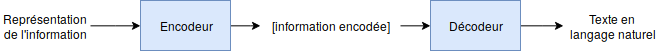
\includegraphics[width=.95\linewidth]{images/NLG/Encoder.png} 
	\caption{Schéma d'une architecture encodeur-décodeur pour NLG} 
\end{figure}
\paragraph{}
Beaucoup d'approches de génération de langage naturel en gestion de dialogue utilisent des encodeurs-décodeurs. \cite{Wen2015} utilisent par exemple des LSTMs sémantiquement conditionnés; ils ajoutent aux LSTMs classiques une couche contenant des informations sur l'action prise par le gestionnaire de dialogue pour assurer que la génération représente le sens désiré. D'autres travaux utilisent des réseaux de neurones récurrents pour encoder l'état du gestionnaire de dialogue et l'entrée reçue, suivie par un décodeur pour générer le texte de la réponse \citep{Sordoni2015,Serban2016,Goyal2016}.
\section{Conclusion}
\paragraph{}
Au terme de ce chapitre et après avoir étudié l'état de l'art sur les systèmes existants, nous avons pu construire un bagage théorique assez complet dans le domaine des SPAs. En assimilant les différentes approches, il est maintenant temps de passer à la conception de notre propre système. Le chapitre suivant introduira nos propositions pour le développement de notre propre SPA qui sera destiné à la manipulation d'un ordinateur.